%! BibTeX Compiler = biber
%TC:ignore
\documentclass{article}

\usepackage{xcolor, colortbl}
\definecolor{BLUELINK}{HTML}{0645AD}
\definecolor{DARKBLUELINK}{HTML}{0B0080}
\PassOptionsToPackage{hyphens}{url}
\usepackage[colorlinks=false]{hyperref}
% for linking between references, figures, TOC, etc in the pdf document
\hypersetup{colorlinks,
    linkcolor=DARKBLUELINK,
    anchorcolor=DARKBLUELINK,
    citecolor=DARKBLUELINK,
    filecolor=DARKBLUELINK,
    menucolor=DARKBLUELINK,
    urlcolor=BLUELINK
} % Color citation links in purple
\PassOptionsToPackage{unicode}{hyperref}
\PassOptionsToPackage{naturalnames}{hyperref}

\usepackage{biorxiv}
\usepackage[backend=biber,style=nature]{biblatex}
\addbibresource{codon_models.bib}

\usepackage{url}
\usepackage{amssymb,amsfonts,amsmath,amsthm,mathtools}
\usepackage{lmodern}
\usepackage{xfrac, nicefrac}
\usepackage{bm}
\usepackage{listings, enumerate, enumitem}
\usepackage[export]{adjustbox}
\usepackage{graphicx}
\usepackage{bbold}
\usepackage{pdfpages}
\pdfinclusioncopyfonts=1
\usepackage{lineno}

\newcommand{\UniDimArray}[1]{\bm{#1}}
\newcommand{\BiDimArray}[1]{\bm{#1}}
\DeclareMathOperator{\E}{\mathbb{E}}
\DeclareMathOperator{\Var}{\mathrm{Var}}
\newcommand{\der}{\mathrm{d}}
\newcommand{\e}{\mathrm{e}}
\newcommand{\avg}[1]{\left< #1 \right>} % for average
\newcommand{\Ne}{N_{\mathrm{e}}}
\newcommand{\proba}{\mathbb{P}}
\newcommand{\pfix}{\proba_{\mathrm{fix}}}
\newcommand{\Spop}{\beta}
\newcommand{\SpopMean}{\overline{\Spop}}
\newcommand{\Sphy}{S}
\newcommand{\SphyMean}{\overline{\Sphy}}
\newcommand{\polyDel}{\proba \left[ {\Spop < -1} \right]}
\newcommand{\polyNeutral}{\proba \left[ -1 < \Spop < 1 \right]}
\newcommand{\polyAdv}{\proba \left[ 1 < \Spop  \right]}

\renewcommand{\baselinestretch}{1.5}
\linenumbers

\title{Empirical evidence for positive selection that is not adaptive evolution}

\author{
    \large
    \textbf{T. {Latrille}$^{1}$, J. {Joseph}$^{2}$, N. {Salamin}$^{1}$}\\
    \normalsize
    $^{1}$Université de Lausanne, Lausanne, Switzerland\\
    $^{1}$Université de Lyon, Lyon, France \\
    \texttt{\href{mailto:thibault.latrille@ens-lyon.org}{thibault.latrille@ens-lyon.org}} \\
}

\begin{document}
    \maketitle

    \begin{abstract}
        Evidence for positive selection occurring in protein-coding DNA sequence is widespread across different taxa.
        Positive selection can be a result of adaptive evolution, meaning that individuals have had to adapt to a change in environment or selective pressure.
        However, current positive selection can also be the result of mutations compensating for deleterious substitutions that have accumulated along lineages, in which case positive selection is non-adaptive and predictable.
        To evaluate the extent of non-adaptive positive selection, we have combined population-genetics and phylogenetics datasets.
        We first leveraged phylogenetic codon models which are based on a population-genetics formalism, assuming a non-adaptive fitness landscape.
        These models estimate the fitness of each of the 20 amino acids for each protein site, given mammalian protein-coding DNA alignments and gene tree topologies.
        Second, we integrated mammalian divergence data with polymorphic variants found in 29 populations across 7 mammalian genera.
        For each non-synonymous variant observed at the population level, we predicted its change in fitness from amino-acid fitnesses estimated at the mammalian scale.
        We found that a large proportion of observed non-synonymous changes are predicted to be positively selected, meaning that the ancestral allele is sub-optimal.
        These supposedly advantageous variants are indeed showing signs of recent positive selection in all populations.
        Our work confirms that deleterious substitutions have accumulated across the phylogeny and are currently being compensated for, resulting in widespread positive selection that is not adaptive evolution.
        This study also shows the leverage obtained by integrating phylogenetic and population genetics on a common formalism.
    \end{abstract}

    \keywords{Selection \and phylogenetic \and population genetics \and codon models}

    Adaptive evolution in proteins can be quantified by comparing sequence variation inside a population to the sequence divergence with a sister species\cite{mcdonald_adaptative_1991}.
    Indeed, strongly adaptive mutations are expected to be observed in substitutions but not in polymorphism because they reach fixation quickly.
    This method has been largely improved to account for possible bias-inducing factors such as the presence of weak positive selection, background selection and demography fluctuations\cite{eyre-walker_distribution_2006, eyre-walker_estimating_2009, galtier_adaptive_2016, tataru_inference_2017}.
    It's application across many taxa has uncovered that a large proportion of substitutions are positively selected\cite{moutinho_variation_2019}.
    In practice, the estimated proportion of fixed substitutions that are positively selected varies from 30\% to 70\% (reference).
    Inside a protein, structural properties such as solvent exposure are positively correlated with the proportion of positively selected substitutions\cite{moutinho_impact_2019}.
    The root causes for this widespread rate of positive selection are however scarcely investigated, often assumed to be the end result of change in the environment or in selection pressure driving individuals to adapt (reference).
    In this view, positive selection is adaptive, such that the underlying fitness landscape is changing with time in response to external constraints, theoretically known as seascape\cite{mustonen_fitness_2009}.
    However, even under the assumption that the fitness landscape is stable, the nearly-neutral theory\cite{ohta_nearly_1992} predicts that positive selection can occur to compensate for deleterious substitutions that have accumulated along lineages.
    Theoretically, at the nearly-neutral equilibrium, the net flow of deleterious and advantageous mutations reaching fixation are equal\cite{sella_application_2005}.
    In other words, mutations are more likely to be deleterious but are less likely to reach fixation, and the total number of fixation are compensated.
    Under this kind of positive selection, advantageous mutations are predictable and evolution is non-adaptive since there is no genetic innovation in response to external constraint, just an advantage to restore a good functioning of proteins\cite{lassig_predicting_2017}.

    Altogether, the goal of this study is to evaluate the extent of non-adaptive positive selection, by combining population-genetics and phylogenetics datasets, and ask a broad range of questions.
    Are proteins optimal?
    Is the fitness landscape stable across the mammalian evolution?
    Can we use phylogenetics to predict the selection coefficient of a mutation?
    Are deleterious mutations reliably purged only when selection overpowers drift?

    A necessary step is being able to estimate fitness landscape on long-term evolution at the phylogenetic scale.
    So called mutation-selection codon models provide a nearly-neutral model of evolution by estimating the fitness landscape over amino-acid sequences, for each site of the sequence\cite{ halpern_evolutionary_1998, rodrigue_mechanistic_2010, tamuri_estimating_2012}.
    Only nearly-neutral mutations between high fitness amino acids will tend to be permitted by the model, allowing for the explicit calculation of the scaled selection coefficient of non-synonymous mutations between codons.
    These models have be used as a null-model to predict the overall rate of evolution of proteins\cite{spielman_relationship_2015, dosreis_how_2015}, from which a departure in the observed overall rate that proteins are evolving under a changing fitness landscape\cite{rodrigue_detecting_2017, tamuri_mutationselection_2021} and is a signal of adaptive evolution\cite{rodrigue_bayesian_2021}.
    Available multiple sequence alignment between mammalian species\cite{ranwez_orthomam_2007, howe_ensembl_2021} are used to estimate fitness landscape on long-term evolution.

    \begin{figure*}[!ht]
        \centering
        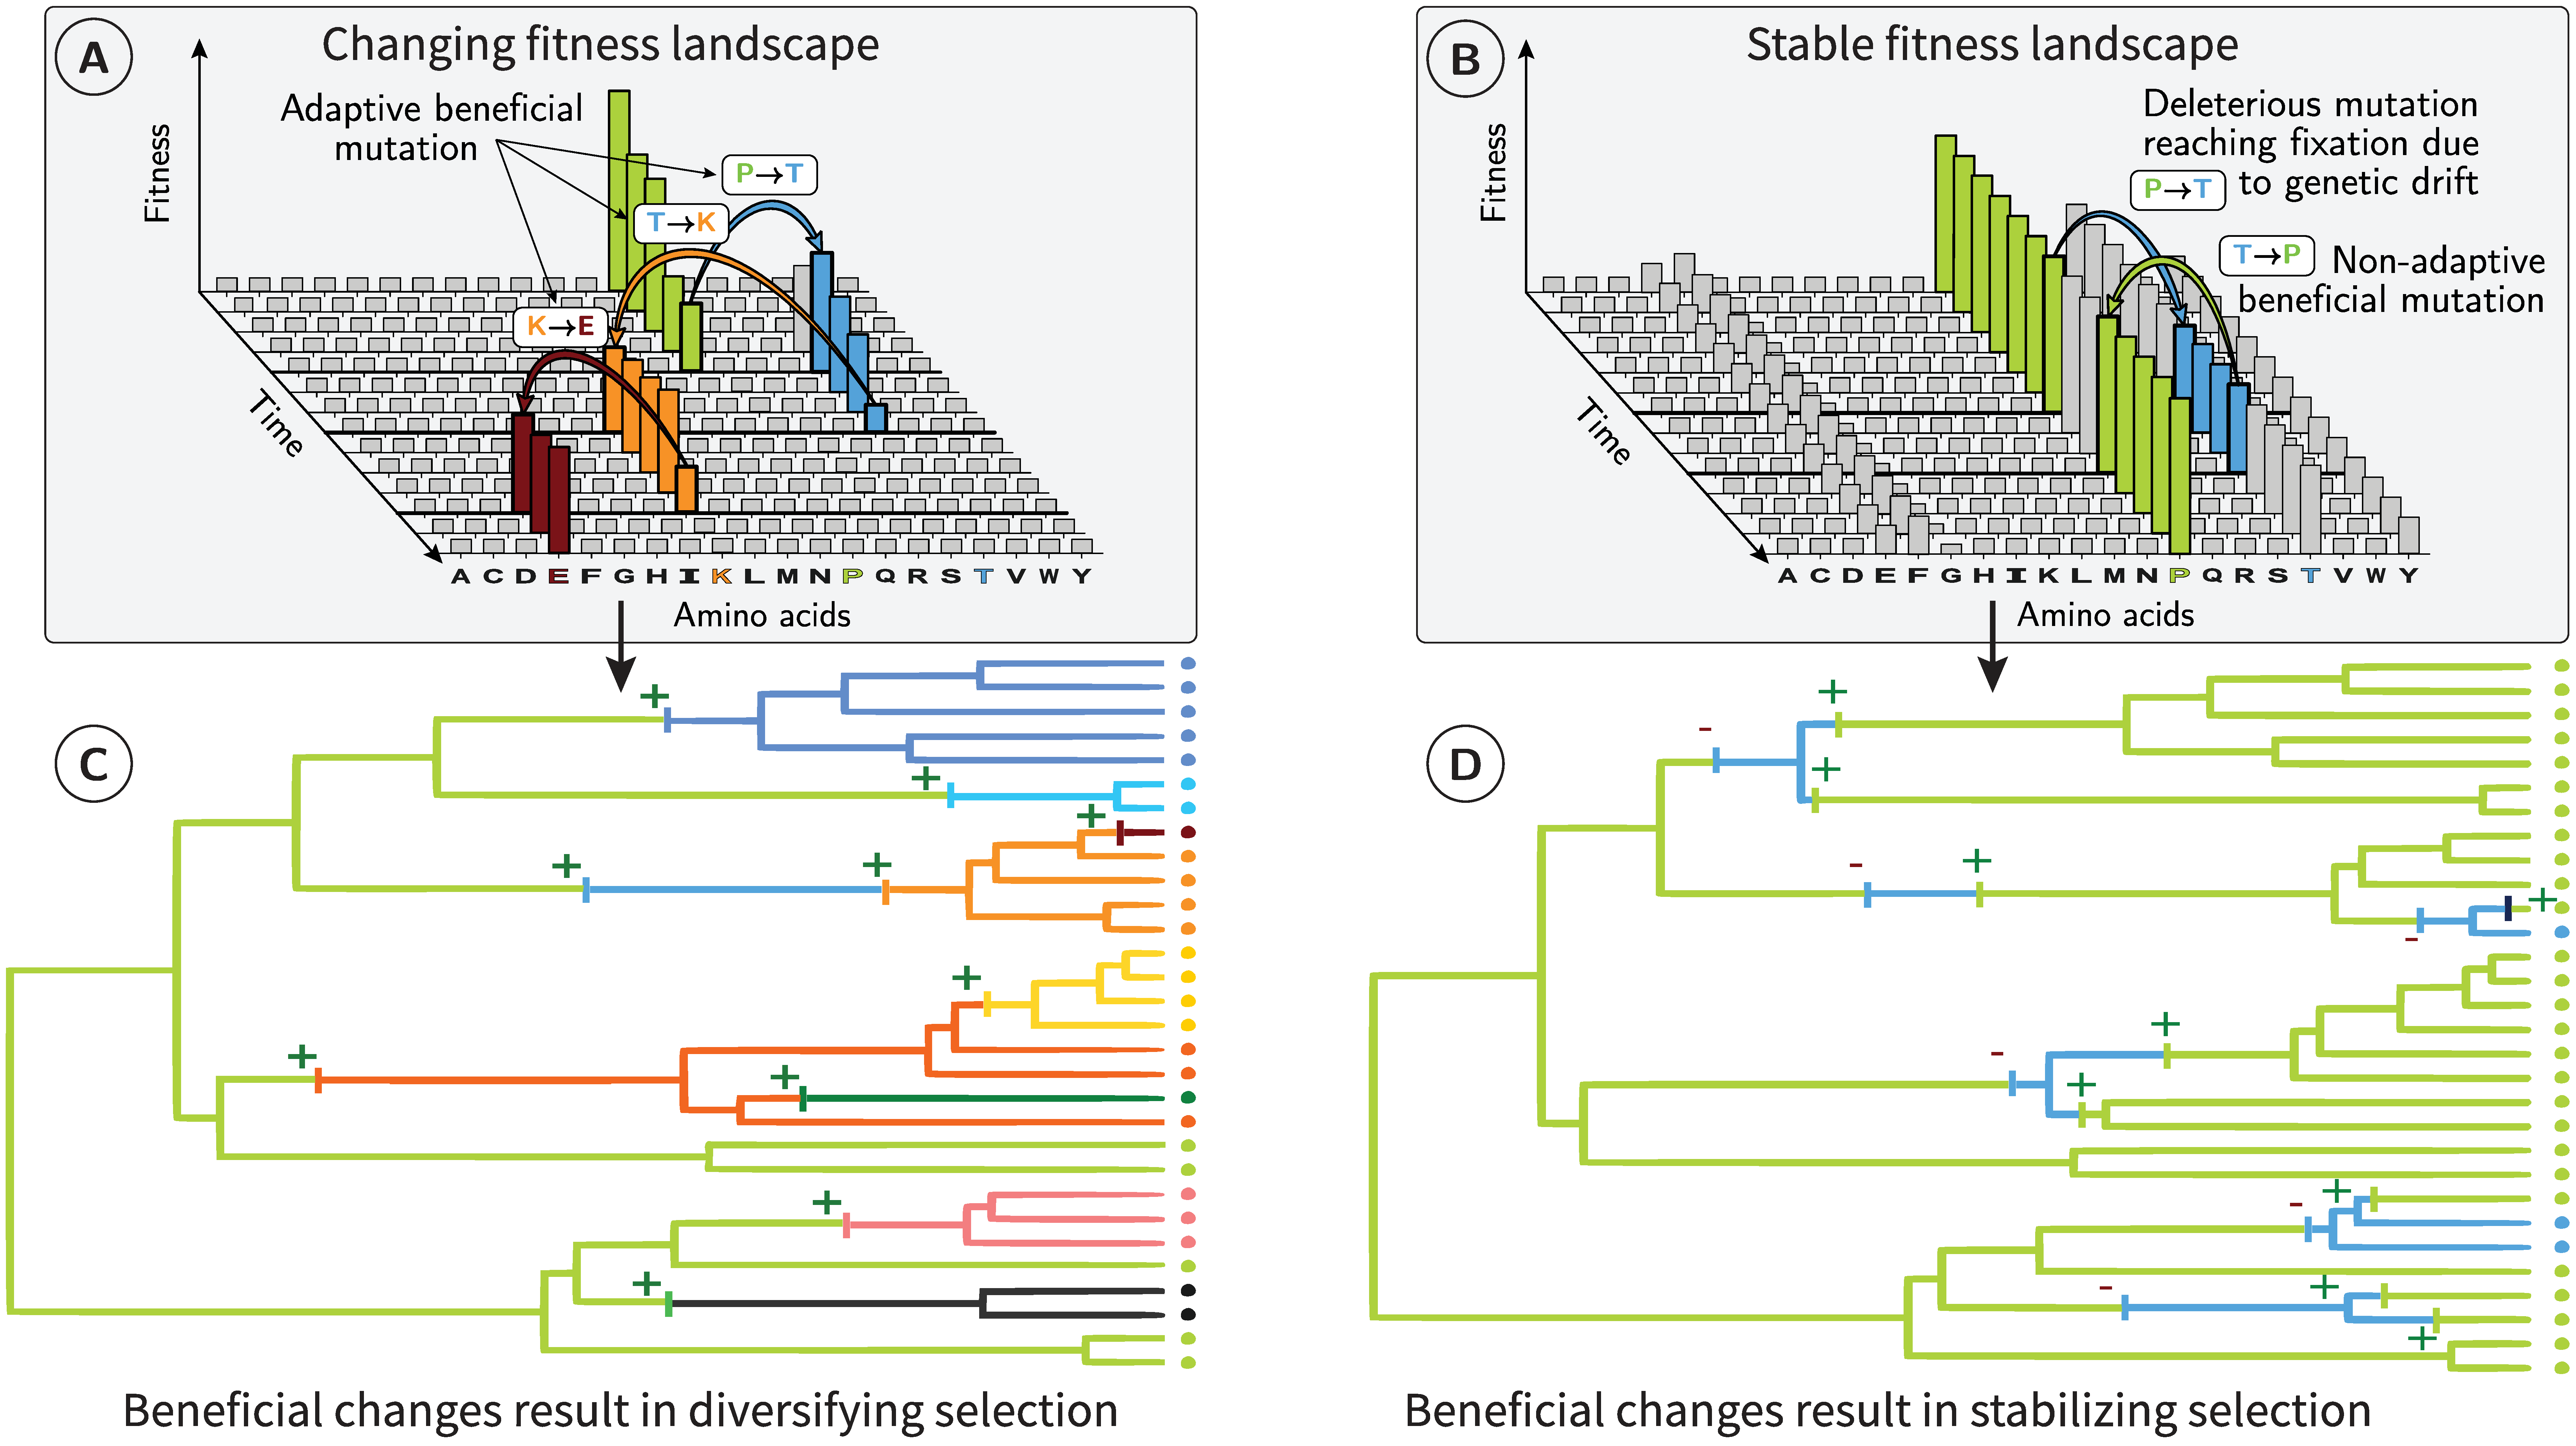
\includegraphics[width=\textwidth, page=1] {artworks/figure1}
        \caption{
            Integrating divergence and polymorphism for the detection of adaptation.
            At the phylogenetic level (panel A), amino-acid Wrightian fitness for each site are estimated from protein-coding DNA alignments using mutation-selection codon models.
            At the population-genetic level (panel B), for each observed single nucleotide polymorphism (SNP), selection coefficient are computed as the difference in amino-acid fitness between the ancestral and derived variant.
        }
        \label{fig:method}
    \end{figure*}

    % How to articulate phylogenetic and population genetic
    This information can be contrasted with the observed variation inside population, such that we can predict the scaled selection coefficient (the change in fitness) for each non-synonymous single nucleotide polymorphism (SNP) observed in a population (fig.~\ref{fig:method}).
    We developed and leveraged a pipeline integrating divergence and polymorphism data across the entire exome for 29 populations across 7 genera, namely \textit{Equus}, \textit{Canis}, \textit{Bos}, \textit{Capra}, \textit{Ovis}, \textit{Chlorocebus} and \textit{Homo}.
    For each non-synonymous SNP observed at the population level, we predicted its scaled selection coefficient ($\Sphy$) in fitness from amino-acid fitness estimated at the mammalian scale (fig.~\ref{fig:homo-afr-results}A).
    Then we ask whether the variants that are supposedly advantageous are showing signature of short term evolution.
    In other words, if a variant is found in many mammals but not in ancestral humans, and a mutation in human is toward the mammal version, is this mutation advantageous for the individual carry it?
    All observed SNPs are divided in 5 classes of selection: severely deleterious with $\Sphy<-3$, deleterious with $-3<\Sphy<-1$, weakly deleterious with $-1<\Sphy<0$, weakly advantageous with $0<\Sphy<1<$ and advantageous with $1<\Sphy$.
    For each class of selection, we first derived its site-frequency spectrum (SFS), which represent the proportion of mutations with a given number of derived allele in the population (fig.~\ref{fig:homo-afr-results}B).
    Compared to synonymous mutations (supposedly neutral), mutations predicted to be advantageous are over-represented at higher frequency, while severally deleterious are under-represented at high frequency, a signature that our prediction are qualitatively in the right direction.
    Aside from the frequency of the derived allele, another information is the total number of observed alleles compared to its expectation, given by the total mutation rate.
    The total mutation rate for each class is computed from the ancestral genome reconstruction (fig.~\ref{fig:homo-afr-results}C).
    For example, for the category of selection with $1<\Sphy$, the expected total mutation rate is obtained by adding together mutation rates for all possible non-synonymous mutations for which the derived allele is toward a fitter amino-acid than the ancestral allele with $\Sphy > 1$.
    The total mutation rate and the SFS are combined to estimate the distribution of the selection coefficient $\Spop$ given by population-based model\cite{tataru_inference_2017, tataru_polydfe_2020}.
    These population based models cannot give a specific estimate of $\Spop$ for each SNP, but by gathering information across many SNPs, these models can estimate the proportion of advantageous mutations ($\polyAdv$), of nearly-neutral mutations ($\polyNeutral$) and of deleterious mutations ($\polyDel$) (fig.~\ref{fig:homo-afr-results}D).


    \begin{figure*}[!ht]
        \centering
        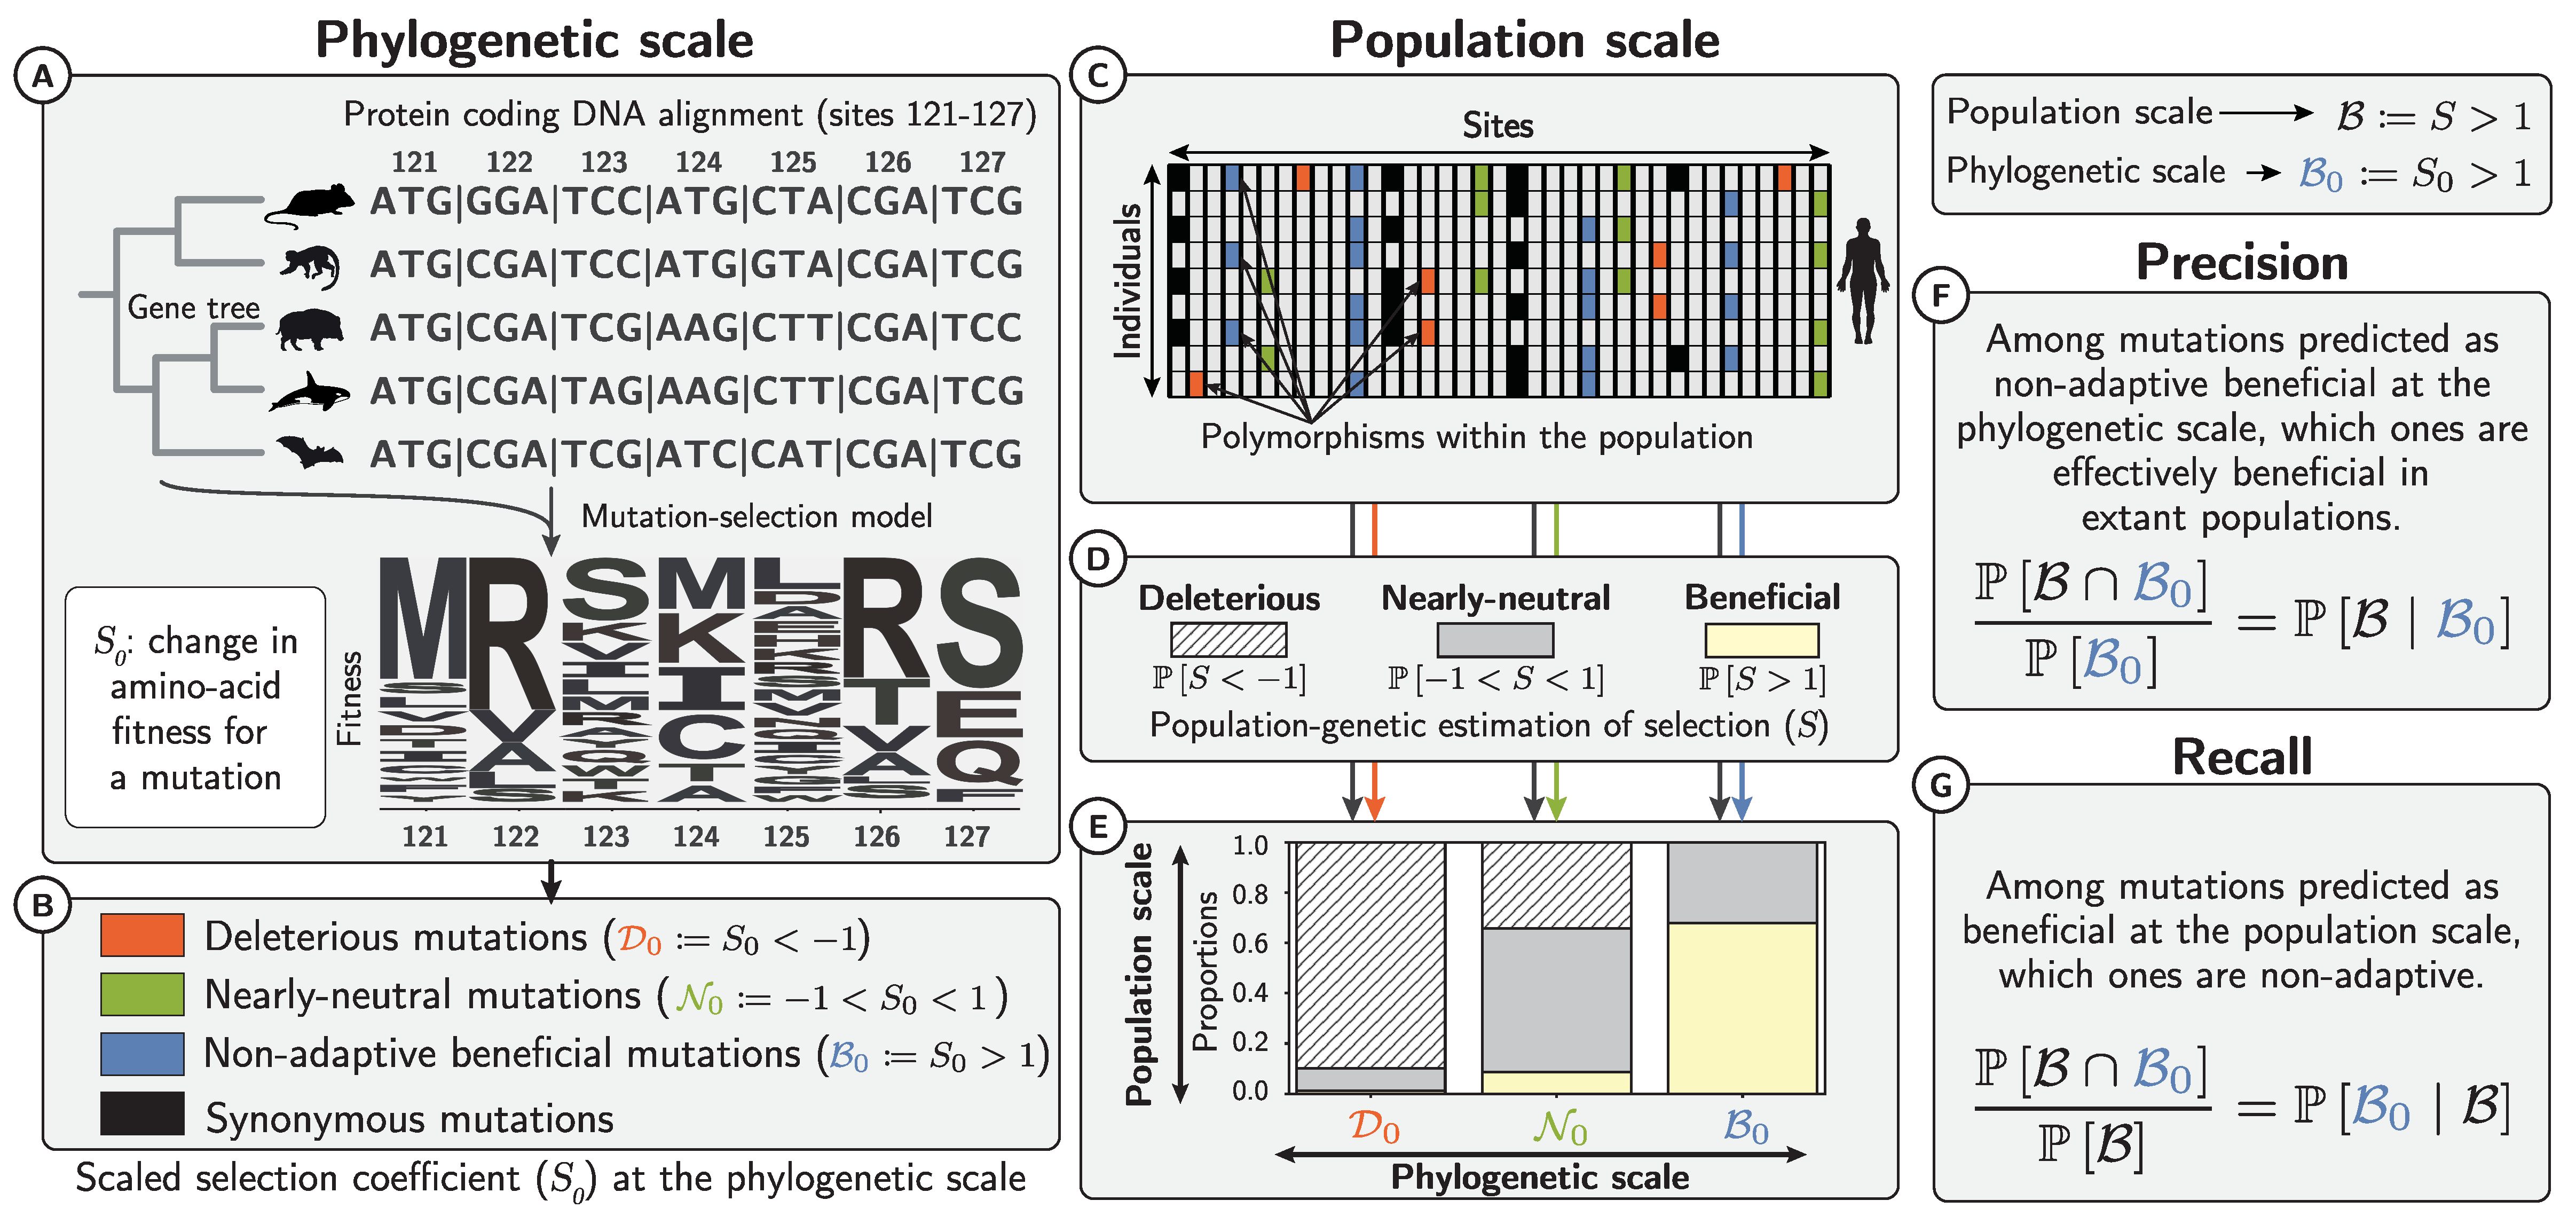
\includegraphics[width=\textwidth, page=1] {artworks/figure2}
        \caption{
            Panel A: Histogram of predicted selection coefficient (S) for each observed mutation in a sample of 512 individuals (1024 alleles) with African descent.
            Mutations are divided in 5 classes of selection: severely deleterious (blue), deleterious (green), weakly deleterious (light green), weakly advantageous (yellow) and advantageous (red).
            Panel B: Site-frequency spectrum (SFS) represent the proportion of mutations (y-axis) with a given number of derived allele in the population (x-axis).
            SFS are drawn for a random sample of 16 alleles (mean in solid line and standard deviation in filled color) for each class of selection and for synonymous mutations supposedly neutral (black).
            Supposedly advantageous are over-represented at higher frequency, while severally deleterious are under-represented at high frequency, a signature of selection.
            Panel C. Histogram of predicted selection coefficient (S) for each possible mutation away from the ancestral human genome, weighted by the mutation rate.
            For each class of selection, the sum of histogram in this class thus gives the expected total mutation rate toward this class.
            If they are less mutations observed than expected, this class is thus undergoing purifying selection.
            Panel D. For each class of selection (and for the set of all non-synonymous mutations), information from the SFS and the expected total mutation rate are combined at the population-genetic scale to estimate the proportion of advantageous mutations $\polyAdv$, of nearly-neutral mutations $\polyNeutral$ and of deleterious mutations $\polyDel$.
        }
        \label{fig:homo-afr-results}
    \end{figure*}

    \begin{figure*}[!ht]
        \centering
        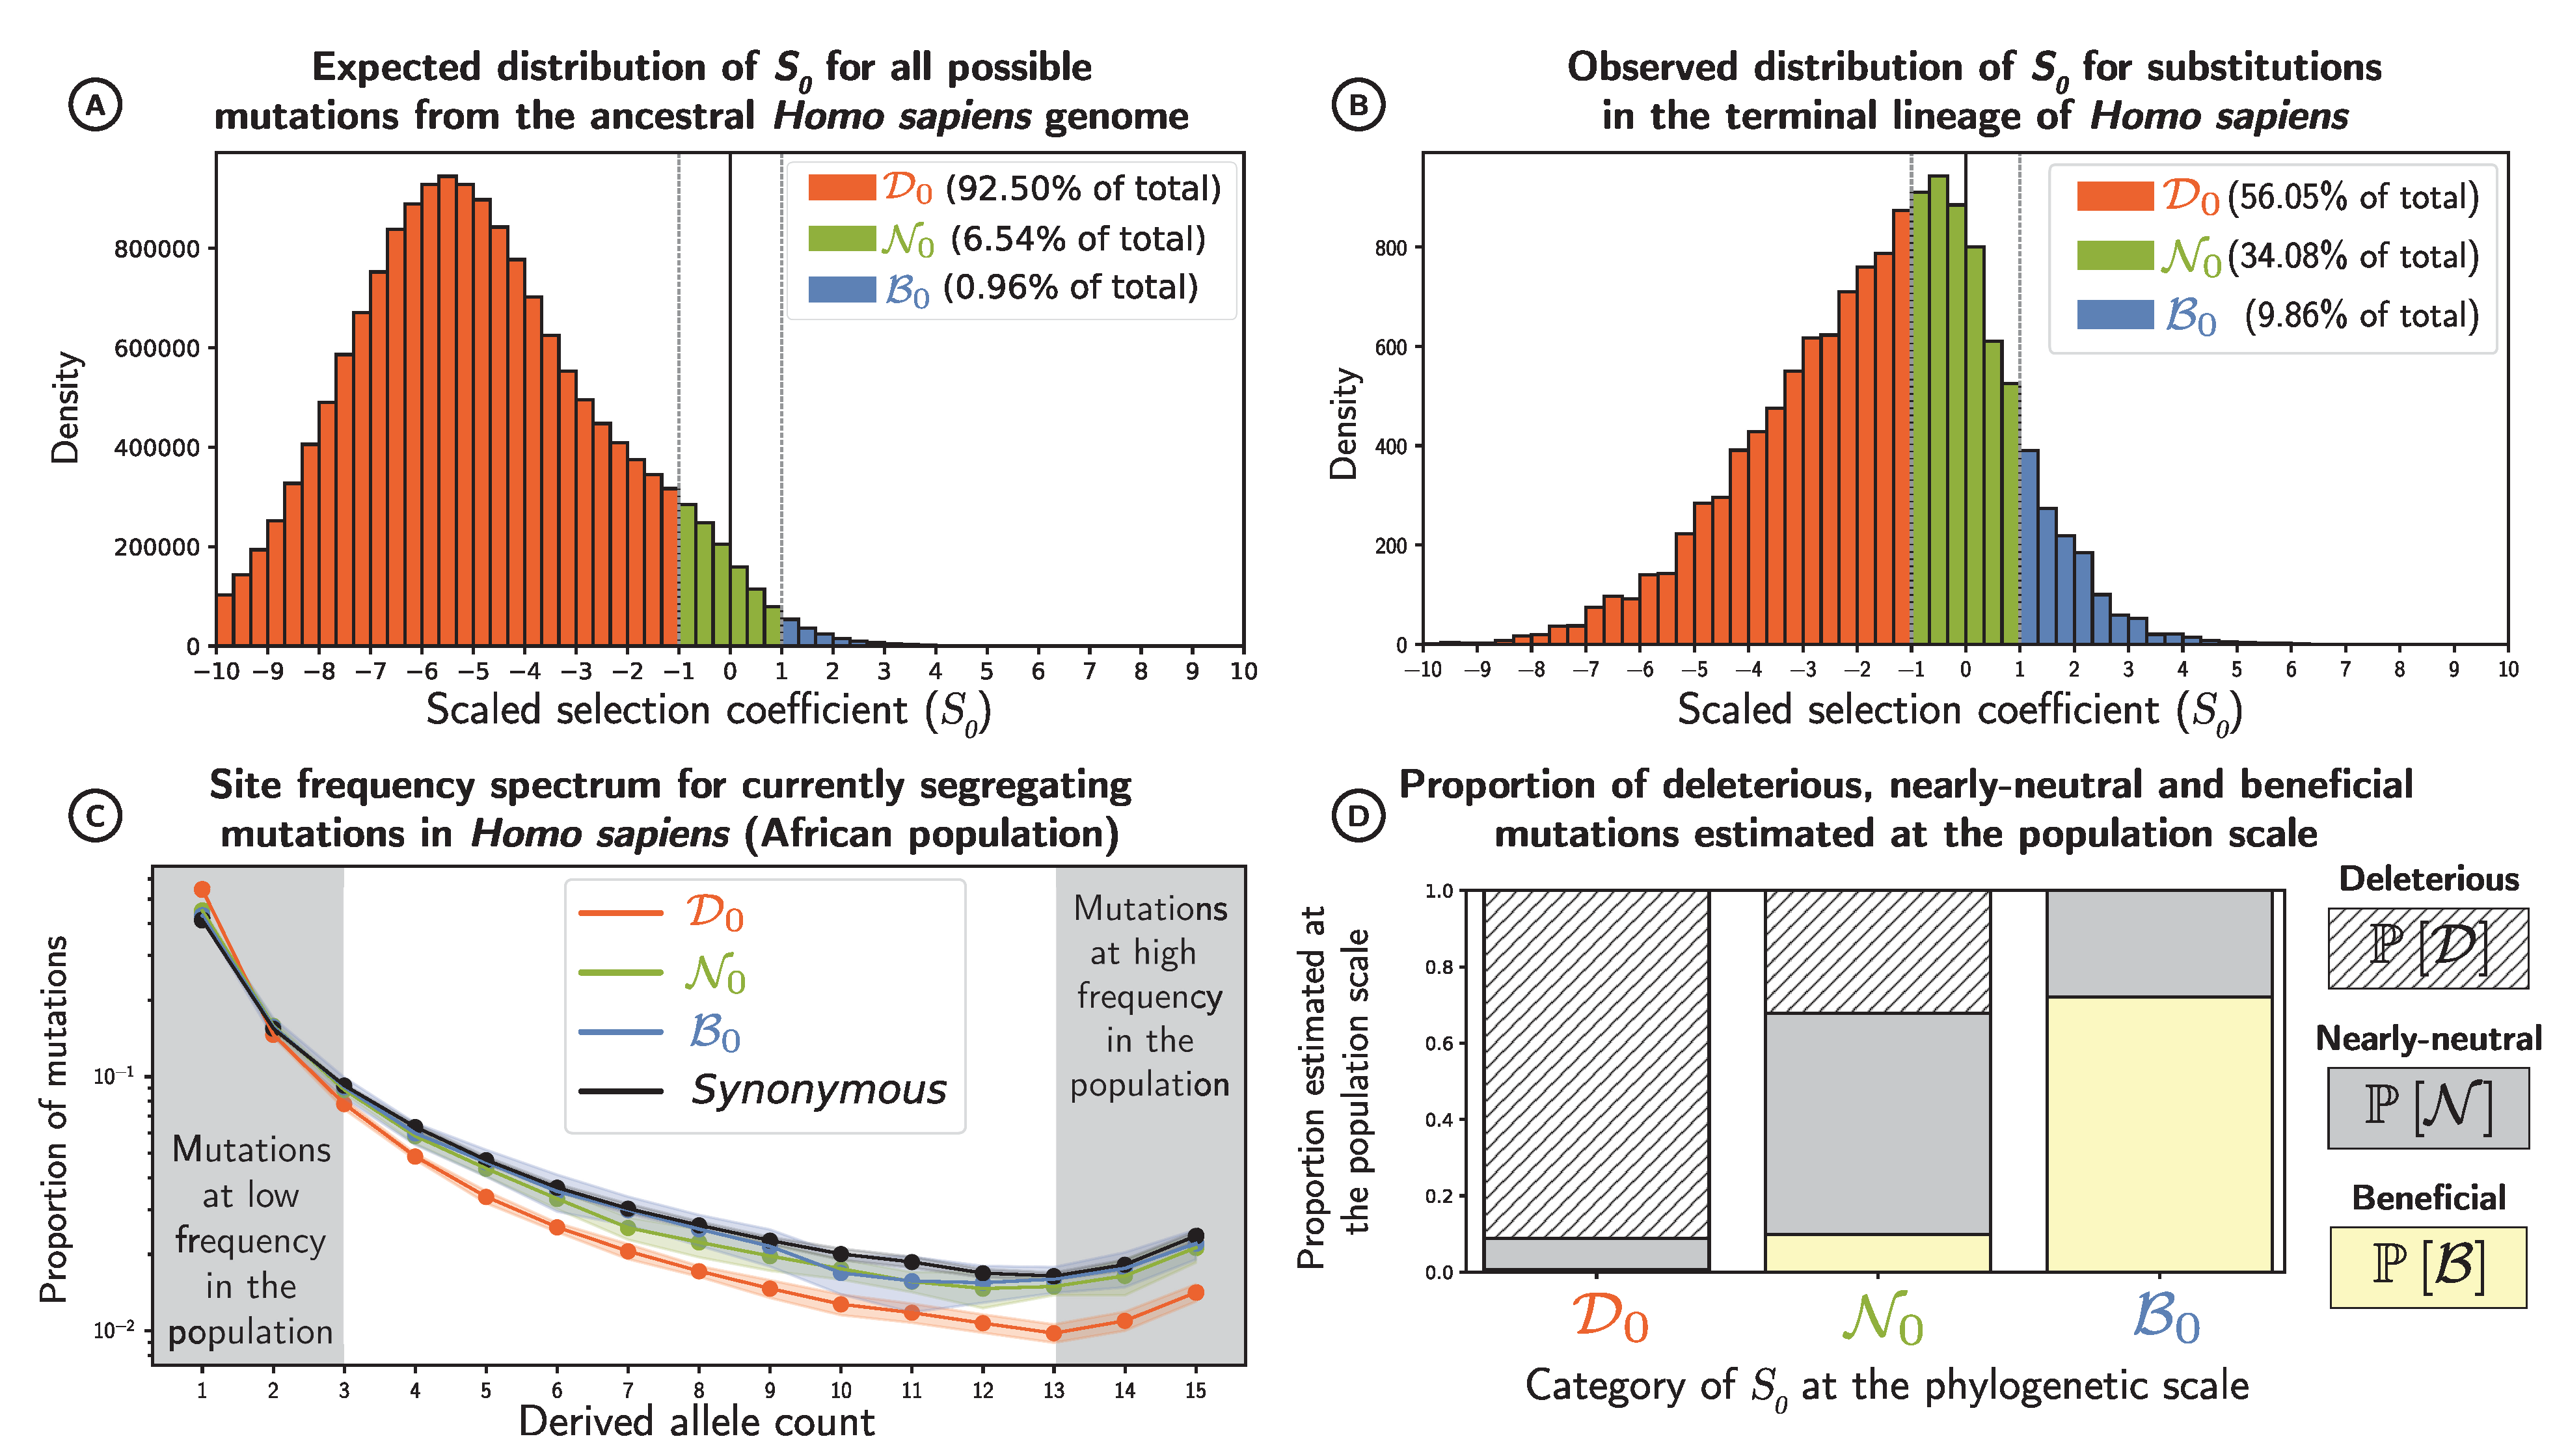
\includegraphics[width=\textwidth, page=1] {artworks/figure3}
        \caption{
            Reproducibility of results shown in figure~\ref{fig:homo-afr-results} in 29 populations across 7 genera.
            From a site-frequency spectrum and total mutation rates are combined at the population-genetic scale to estimate the proportion of advantageous mutations $\polyAdv$ in top panel, of nearly-neutral mutations $\polyNeutral$ in middle panel and of deleterious mutations $\polyDel$ in bottom panel.
        }
        \label{fig:all-pop-results}
    \end{figure*}

    Because of this observed overlap between phylogenetic and population-genetic methods, both estimating a scaled selection coefficient, we could study the estimation of the mean $\SpopMean$ as a function of the mean $\SphyMean$.
    However, the mean selection coefficient estimated at the phylogenetic scale is usually drastically negative because of the heavy tail of the negative part of the estimated DFE.
    Hence we focused on the relationship between $\SpopMean$ and $\SphyMean$ for a subset of SNPs, for which $\SphyMean$ is close to $0$.
    Sliding window of groups of $5.000$ SNPs are taken with a mean $\SphyMean$ between $-0.5$ and $0.5$ (fig.~\ref{fig:selcoeff-pop-phylo}A).
    $\SpopMean$ is estimated for each group, with some groups that might have part of same SNPs that overlap.
    The relationship between $\SpopMean$ and $\SphyMean$ is best described as a second order polynomial, and the slope of this polynomial at $\SphyMean=0$ gives the ratio $\SpopMean/\SphyMean$ for each population.
    We observ that $\SpopMean/\SphyMean$, representing the efficiency of selection at the short versus long term is positively correlated with synonymous diversity, a proxy of effective population siz.
    Altogether, population with large effective population size are under more efficient selection.

    \begin{figure*}[!ht]
        \centering
        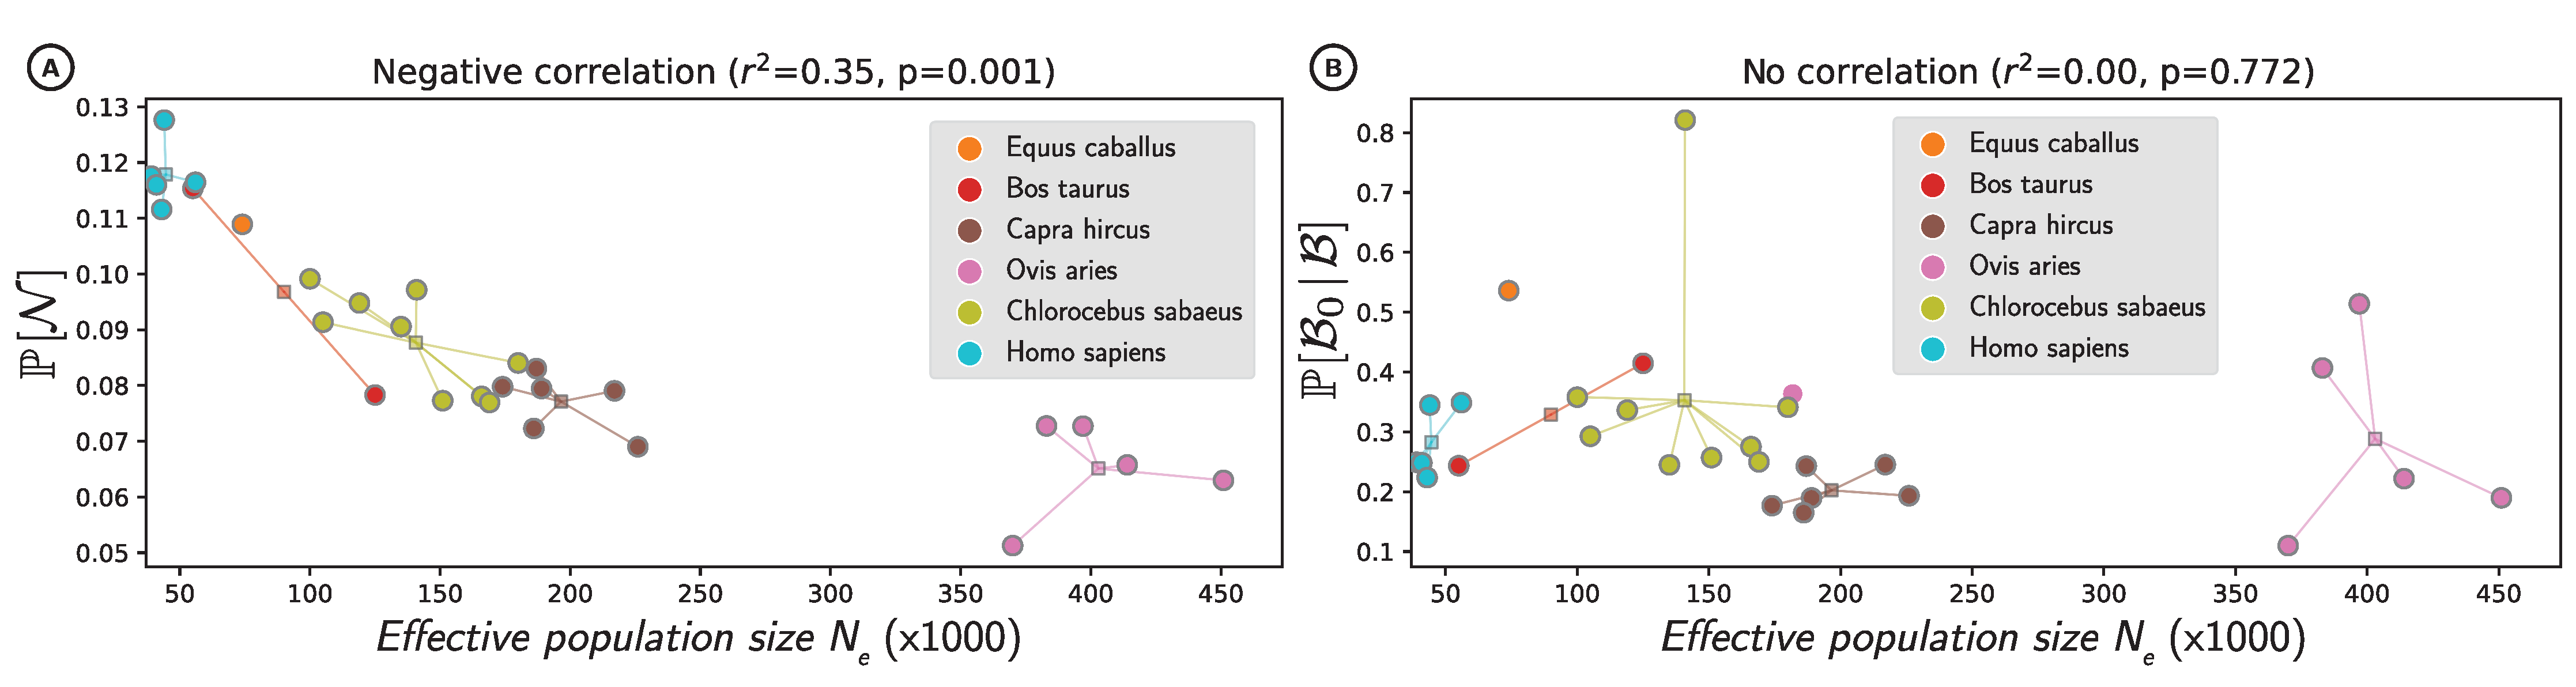
\includegraphics[width=\textwidth, page=1] {artworks/figure4}
        \caption{
            Panel A. For each population, proportion of advantageous ($\polyAdv$), nearly-neutral ($\polyNeutral$) and of deleterious ($\polyDel$) mutations estimated at the population-genetic scale.
            Estimation is performed with SNPs predicted to be weakly-advantageous at the phylogenetic scale $0<\Sphy<1<$.
            Panel B. Mean selection coefficient at the population scale $\SpopMean$ as a function of phylogenetic $\SphyMean$.
            Observed SNPs are sorted and groups of $5.000$ SNPs are taken as a sliding windows with increasing mean $-0.5 \leq \SphyMean \leq 0.5$.
            For each group along the sliding window, $\SpopMean$ (y-axis) is estimated based on SFS and the total mutation rate, and compared to the mean $\SphyMean$ (x-axis).
            A second order polynomial is fitted for each population, and the slope of this polynomial at $\SphyMean=0$ gives the ratio $\SpopMean/\SphyMean$ given in legend.
            Panel C. Ratio $\SpopMean/\SphyMean$ as a function of the synonymous diversity for each population.
            Populations with higher diversity are showing higher ratio of ratio $\SpopMean/\SphyMean$.
        }
        \label{fig:selcoeff-pop-phylo}
    \end{figure*}

    % Our study is a bridge between phylogenetic and population genetics
    From a theoretical evolution perspective, we found that we could use phylogenetics to predict the selection coefficient of a mutation.
    Appart from phylogenetic mutation-selection codon models, SIFT scores based on amino-acid alignments across species have already be found to be informative of the selection pressure exerted at the population scale\cite{chen_hunting_2021}.
    However, they do not integrate the underlying phylogeny nor the underlying mutational process.
    Additionally, they are not based on population-genetics formalism, hence the relationship between selection coefficient and SIFT score is not straightforward.
    We found here that mutation-selection formalism greatly outperforms SIFT score to predict the selection coefficient of mutations (Supplementary Materials).
    Most importantly, we showed that mutation-selection codon models formalize a bridge between phylogenetics and population genetics.
    Our study is a bridge between phylogenetic and population genetics, but both ends has its limitation.

    % Problem with the current mutation-selection model, and the way forward
    For phylogenetic models, current mutation-selection codon model are sensitive to mis-alignment.
    They are also assuming no changes in effective population size\cite{latrille_inferring_2021}.
    Epistasis is not modelled while it can have drastic consequence on the change in fitness landscape\cite{latrille_quantifying_2021}.
    However, both relaxation are computationally intensive, and would require new mutation-selection models and optimization techniques to be able to manipulate genome-wide datasets.
    For population-genetic model, the distribution of fitness effects have so far been assumed to be constrained by
    The DFE is assumed to be a gamma-distribution for deleterious mutations and an exponential for advantageous mutations, thus implicitly assuming a peak around 0.
    The DFE predicted from fitness landscapes are very different, with peak is shifted toward negatively selected mutations.
    Moreover, these methods estimate selection coefficient that are very negative on average, which is not biologically sensible.
    Altogether, we should seek to reproduce our experiment with other clades, such as drosophila, birds and with for more shallow but wider phylogeny to determine the extend of reproducibilty of our results.

    % We should take that into account.
    From a structural biology perspective, we found that proteins are not optimal, with a large proportion of mutations still toward more optimal amino acids.
    Seen from another angle, it means that we could theoretically derive the fittest proteins using only the amino acid with the highest fitness.
    We could then test whether fittest proteins are also thermodynamically more stable, leveraging recent developments able to compute efficiently and accurately the folding of proteins.
    From an evolutionary biology perspective, we found that the fitness landscape is relatively stable across the mammalian evolution.
    Mutations with $\Sphy<-1$ are more strongly purged, mutations with $1<\Sphy$ are more often segregating.
    However, how to reliably quantify the overlap between phylogenetic and population-genetic methods?
    The DFE has indeed be found to be reliably constant between species\cite{castellano_comparison_2019}.
    Are deleterious mutations reliably purged only when selection overpowers drift?
    Yes, mutations with predicted $-1<\Sphy<1$ are equivalent to neutral mutations.


    \section*{Acknowledgment}
    \label{sec:acknowledgment}
    We gratefully acknowledge the help of Nicolas Lartillot for his advice and review concerning this manuscript.
    This work was performed using the computing facilities of the CC LBBE/PRABI\@.
    \textbf{Funding:}
    Université de Lausanne;
    French National Research Agency, Grant ANR-19-CE12-0019 / HotRec.
    \textbf{Author contributions:}
    Original idea: T.L.\ and J.J.;
    Model conception: T.L., J.J.\ and N.S.;
    Code: T.L.;
    Data analyses: T.L.\ and J.J.;
    Interpretation: T.L., J.J.\ and N.S.;
    First draft, editing and revisions: T.L., J.J.\ and N.S.;
    Project management and funding: N.S\@.
    \textbf{Competing interests:}
    The authors declare no conflicts of interest.
    \textbf{Data and materials availability:}
    Snakemake pipeline, analysis scripts and documentations are available at \href{https://github.com/ThibaultLatrille/SelCoeff}{github.com/ThibaultLatrille/SelCoeff}.


    \section{Material \& Methods}
    \label{sec:methods}

    \subsection{Phylogenetic dataset}

    Protein-coding DNA sequences alignments in placental mammals are extracted from the \href{https://www.orthomam.univ-montp2.fr}{OrthoMaM} database\cite{ranwez_orthomam_2007, douzery_orthomam_2014, scornavacca_orthomam_2019}.
    Genes located on the X, Y and mitochondrial chromosome are discarded from the analysis, since the number of polymorphism, necessary in population-based method, is expected to be different on these sequences.
    Additionally, sequences from the species for which polymorphism are available, as well as their sister species have been discarded from the analysis to ensure independence between the data used in the phylogenetic and population-genetic method.

    \subsection{Selection coefficient (S) in phylogeny-based method}
    \label{subsec:s-phylogeny-method}

    Mutation-selection models assume that the protein-coding sequence is at mutation-selection balance under a fixed fitness landscape, which is itself characterized by a fitness vector over the $20$ amino-acid at each site\cite{yang_mutationselection_2008, halpern_evolutionary_1998, rodrigue_mechanistic_2010}.
    Mathematically, the rate of non-synonymous substitution from codon $a$ to codon $b$ ($q_{a \mapsto b}^{(i)}$) at site $i$ of the sequence is equal to the rate of mutation from the underlying DNA change ($\mu_{a \mapsto b}$) multiplied by the scaled probability of fixation of the mutation ($\proba_{a \mapsto b}^{(i)}$).
    Crucially, the probability of fixation depends on the difference of scaled fitness between the amino-acid encoded by the mutated codon ($F_b^{(i)}$) and the fitness of the amino-acid encoded by the original codon ($F_a^{(i)}$) of site $i$\cite{wright_evolution_1931, fisher_genetical_1930}.
    Altogether, the rate of substitution from codon $a$ to $b$ at a given site $i$ is:
    \begin{equation}
        q_{a \mapsto b}^{(i)} = \mu_{a \mapsto b} \proba_{a \mapsto b}^{(i)} = \mu_{a \mapsto b} \dfrac{F_b^{(i)} - F_a^{(i)}}{1 - \e^{F_a^{(i)} - F_b^{(i)}}}.\label{eq:equation}
    \end{equation}
    Fitting the mutation-selection model on a sequence alignment leads to an estimation of the mutation rate matrix ($\UniDimArray{\mu}$) as well as the 20 amino-acid fitness landscape ($\UniDimArray{F^{(i)}}$) at each site $i$.
    We ran the Bayesian software \href{https://github.com/bayesiancook/bayescode}{BayesCode} on each protein-coding DNA alignment\cite{lartillot_phylobayes_2013, rodrigue_detecting_2017}.
    Each Monte-Carlo Markov-Chain (MCMC) is run during $2000$ points, with a burn-in of $1000$ points, allowing to compute the mean amino-acid fitness landscape ($\UniDimArray{F^{(i)}}$) at each site $i$ across the MCMC\@.

    \subsection{Polymorphism dataset}
    \label{subsec:polymorphism-dataset}

    In order to compare polymorphism and divergence, each SNP (chromosome, position, strand) in the focal species must be matched to its relative position in the protein-coding DNA alignment.
    First, genomic positions are converted to relative position in the coding sequence (CDS) using gene annotation files (GTF format) downloaded from Ensembl (\url{ensembl.org}), we verified the SNP match the reference in the CDS (FASTA format) also downloaded from Ensembl.
    Secondly, relative position in the CDS is converted to position in the multiple sequence alignment (containing gaps) from OrthoMaM database\cite{ranwez_orthomam_2007, douzery_orthomam_2014, scornavacca_orthomam_2019} by doing a global pairwise alignment (Biopython pairwise2) between the CDS fasta and the sequence found in the alignment.
    This conversion from genomic position to position in the alignment is only possible if the assembly used for SNP calling is the same as the one used in the alignment, the GTF annotations and the FASTA sequences.
    We retrieved polymorphism from different projects.
    \textit{Equus caballus} variants called on the EquCab2 assembly in the EVA study PRJEB9799.
    \textit{Canis familiars} variants called on the CanFam3.1 assembly in the EVA study PRJEB24066.
    \textit{Bos taurus} variants called on the UMD3.1 assembly in the next-gen project.
    \textit{Ovis aries} variants called on the Oar\_v3.1 assembly in the next-gen project.
    \textit{Capra Hircus} variants called on the CHIR1 assembly in the next-gen project, we performed a liftover to the ARS1 assembly.
    \textit{Chlorocebus sabaeus} variants are called on the ChlSab1.1 assembly in the EVA study PRJEB22989\cite{svardal_ancient_2017}.
    \textit{Homo sapiens} variants are called on the GRCh38 assembly in the 1000-genome project\cite{consortium_integrated_2012, the1000genomesprojectconsortium_global_2015}.
    Variants not inside genes are discarded at the beginning of the analysis.
    Insertions and deletions are not analyzed, and only Single Nucleotide Polymorphisms (SNPs) with only one mutant allele are considered.
    Stop codon mutants are also discarded.
    For populations containing more than $8$ sampled individuals, the site-frequency spectrum (SFS) is sub-sampled down to $16$ chromosomes ($8$ diploid individuals) without replacement (hyper-geometric distribution) to alleviate the effect of different sampling depth in the $29$ populations.
    SNPs are polarized using the $3$ closest out-groups found in the OrthoMam alignment with est-usfs\cite{keightley_inferring_2018}.
    The Snakemake pipeline for integrating polymorphism and divergence data uses custom scripts written in python 3.8.

    \subsection{Selection coefficient ($\Spop$) in population-based method}
    \label{subsec:s-polymorphism-method}
    The probability to sample allele at a given frequency (before fixation or extinction) is informative of its scaled selection coefficient at the population-scale ($\Spop$).
    Pooled across many sites, the SFS is thus informative on the underlying $\Spop$ of mutations, given we have a neutral expectation.
    In this configuration, a single $\Spop$ for all sampled mutations is biologically not realistic.
    Accordingly, a distribution of fitness effects of mutations (DFE) is assumed, usually modelled as a continuous distribution\cite{eyre-walker_distribution_2006, eyre-walker_estimating_2009}.
    In this study, we used the software polyDFE\cite{tataru_inference_2017, tataru_polydfe_2020}, for which the DFE ($\phi$) is given by a mixture of a $\Gamma$ and Exponential distributions, parameterized by $\Spop_d$ , $b$, $p_b$
    and $\Spop_b$ as:
    \begin{equation*}
        \phi \left( \Spop; \Spop_d , b, p_b, \Spop_b \right) =
        \begin{dcases}
            \left( 1 - p_b \right) f_{\Gamma}(-\Spop; -\Spop_d, b) & \text{ if $\Spop \leq 0$,} \\
            p_b f_{e}(\Spop; \Spop_b) & \text{ if $\Spop > 0$,} \\
        \end{dcases}
    \end{equation*}
    where $\Spop_d < 0 $ is the mean of the DFE for $\Spop \leq 0$,
    $b > 0$ is the shape of the $\Gamma$ distribution,
    $0 \leq p_b \leq 1$ is the probability that $\Spop > 0$,
    $\Spop_b > 0$ is the mean of the DFE for $\Spop > 0$,
    and $f_{\Gamma}(x; m, b)$ is the density of the $\Gamma$ distribution with mean m and shape b, while $f_{e}(x; m)$ is the density of the Exponential distribution with mean $m$.
    Once the DFE is fitted to the data, the proportion of advantageous ($\polyAdv$), nearly-neutral ($\polyNeutral$) and deleterious mutations ($\polyDel$) are given as:
    \begin{align*}
        \polyAdv &= p_b \int_{1}^{+\infty} f_{e}(\Spop; \Spop_b) \der \Spop  \\
        \polyNeutral &= p_b \int_{0}^{1} f_{e}(\Spop; \Spop_b) \der \Spop + \left( 1 - p_b \right) \int_{0}^{1} f_{\Gamma}(\Spop; -\Spop_d, b) \der \Spop \\
        \polyDel &= \left( 1 - p_b \right) \int_{1}^{+\infty} f_{\Gamma}(\Spop; -\Spop_d, b) \der \Spop
    \end{align*}
    And finally, the mean of the DFE $\overline{\Spop}$ is given by:
    \begin{align*}
        \SpopMean & = \int_{-\infty}^{+\infty} \Spop \phi \left( \Spop; \Spop_d , b, p_b, \Spop_b \right) \der \Spop \\
        & =  p_b \Spop_b + \left( 1 - p_b \right) \Spop_d
    \end{align*}
    PolyDFE requires one SFS for non-synonymous mutations and one for synonymous mutations (neutral expectation), as well as the total mutation rate (mutation rate per site multiplied by number of sites) on which each SFS has been sampled.
    The total mutation rate for each SFS is thus obtained using the following three-steps procedure.
    First, for each gene, the reference DNA sequence is adjusted with ancestral and fixed polymorphism for each population.
    Second, from this reconstructed sequence, all possible mutations are computed, weighted by the mutation rate between nucleotide estimated at the phylogenetic scale $\UniDimArray{\mu}$.
    Third, these possible mutation are then classified whether they are synonymous or non-synonymous (stop mutations are excluded), non-synonymous mutations are then also classified depending on their selection coefficient ($\Sphy$).
    From the SFS and the total mutation rate for the both synonymous and for the class of non-syonymous, polyDFE estimates the DFE $\phi$ using maximum likelihood.\@.

    \printbibliography
\end{document}